\section{User insertion}
Only the university and the admins can create new users.

Inserting an user in the system is an operation that has two phases: 
\begin{itemize}
\item The first one requires that the university (or an admin) creates a new account in the system inserting the fiscal code of the user and an unique code (as in Figure~\ref{fig:userInsertionAdmin});
\begin{figure}[!h]
	\centering
	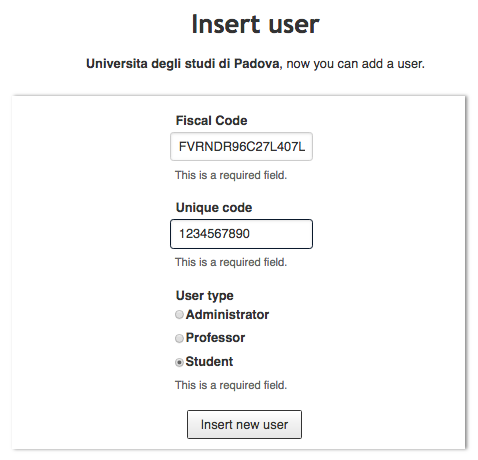
\includegraphics[width=0.60\textwidth, height=3in]{img/userInsertionAdmin.png}
	\caption{User insertion by an admin or university}
	\label{fig:userInsertionAdmin}
\end{figure}

\item The second one is necessary to authenticate and identify the new user: in fact, the  new user during the Sign Up will have to insert its own Fiscal Code and the Identification Code issued by the university (or an admin), and other data as in Figure~\ref{fig:stdSignUp}. If this two data (Fiscal Code and Identification Code) are the same as those inserted by the University (or an admin), then all  the user's personal data will be saved and its Metamask address connected to the account, so that the next logins can be made automatically.
If the form has been filled correctly, than a Metamask window will be opened in front of you. Confirm clicking the \textbf{SUBMIT} button.
\begin{figure}[!h]
	\centering
	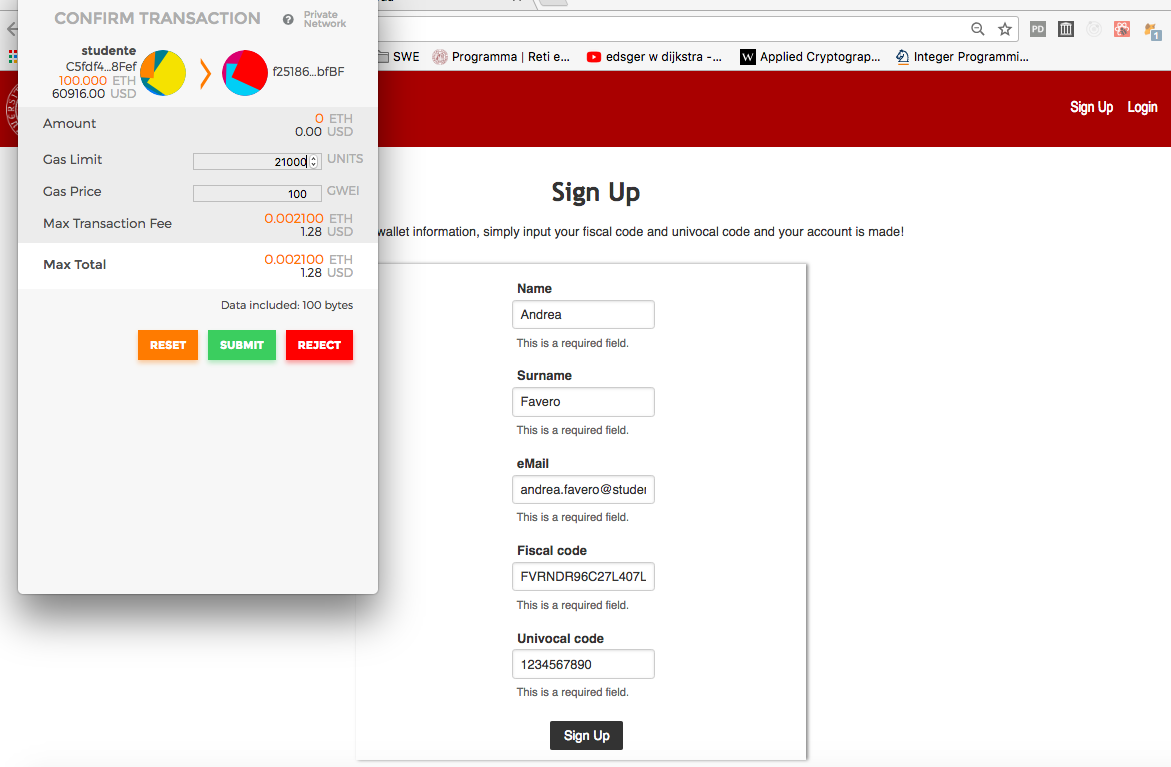
\includegraphics[width=0.65\textwidth]{img/studentInsertion.png}
	\caption{User Sign Up}
	\label{fig:stdSignUp}
\end{figure}
\end{itemize}
